% Fig 4.3 - INITIAL architecture (predict-then-optimize / packed-slot design).
% Standalone -> tight-bbox vector PDF, included by main.tex via \includegraphics.
% Compile: pdflatex arch_initial.tex
\documentclass[border=12pt]{standalone}
\usepackage[T1]{fontenc}
\usepackage{helvet}
\renewcommand{\familydefault}{\sfdefault}
\usepackage{tikz}
\usetikzlibrary{positioning,fit,backgrounds,arrows.meta,shapes.geometric,calc}

\definecolor{blueStroke}{HTML}{1D4ED8}
\definecolor{blueFill}{HTML}{EFF6FF}
\definecolor{paFill}{HTML}{EAF2FE}
\definecolor{purpStroke}{HTML}{6D28D9}
\definecolor{purpFill}{HTML}{FAF5FF}
\definecolor{greenStroke}{HTML}{047857}
\definecolor{greenFill}{HTML}{ECFDF5}
\definecolor{amber}{HTML}{B45309}
\definecolor{amberFill}{HTML}{FEF3C7}
\definecolor{slate}{HTML}{475569}
\definecolor{slateFill}{HTML}{F1F5F9}
\definecolor{inkText}{HTML}{1F2937}

\begin{document}
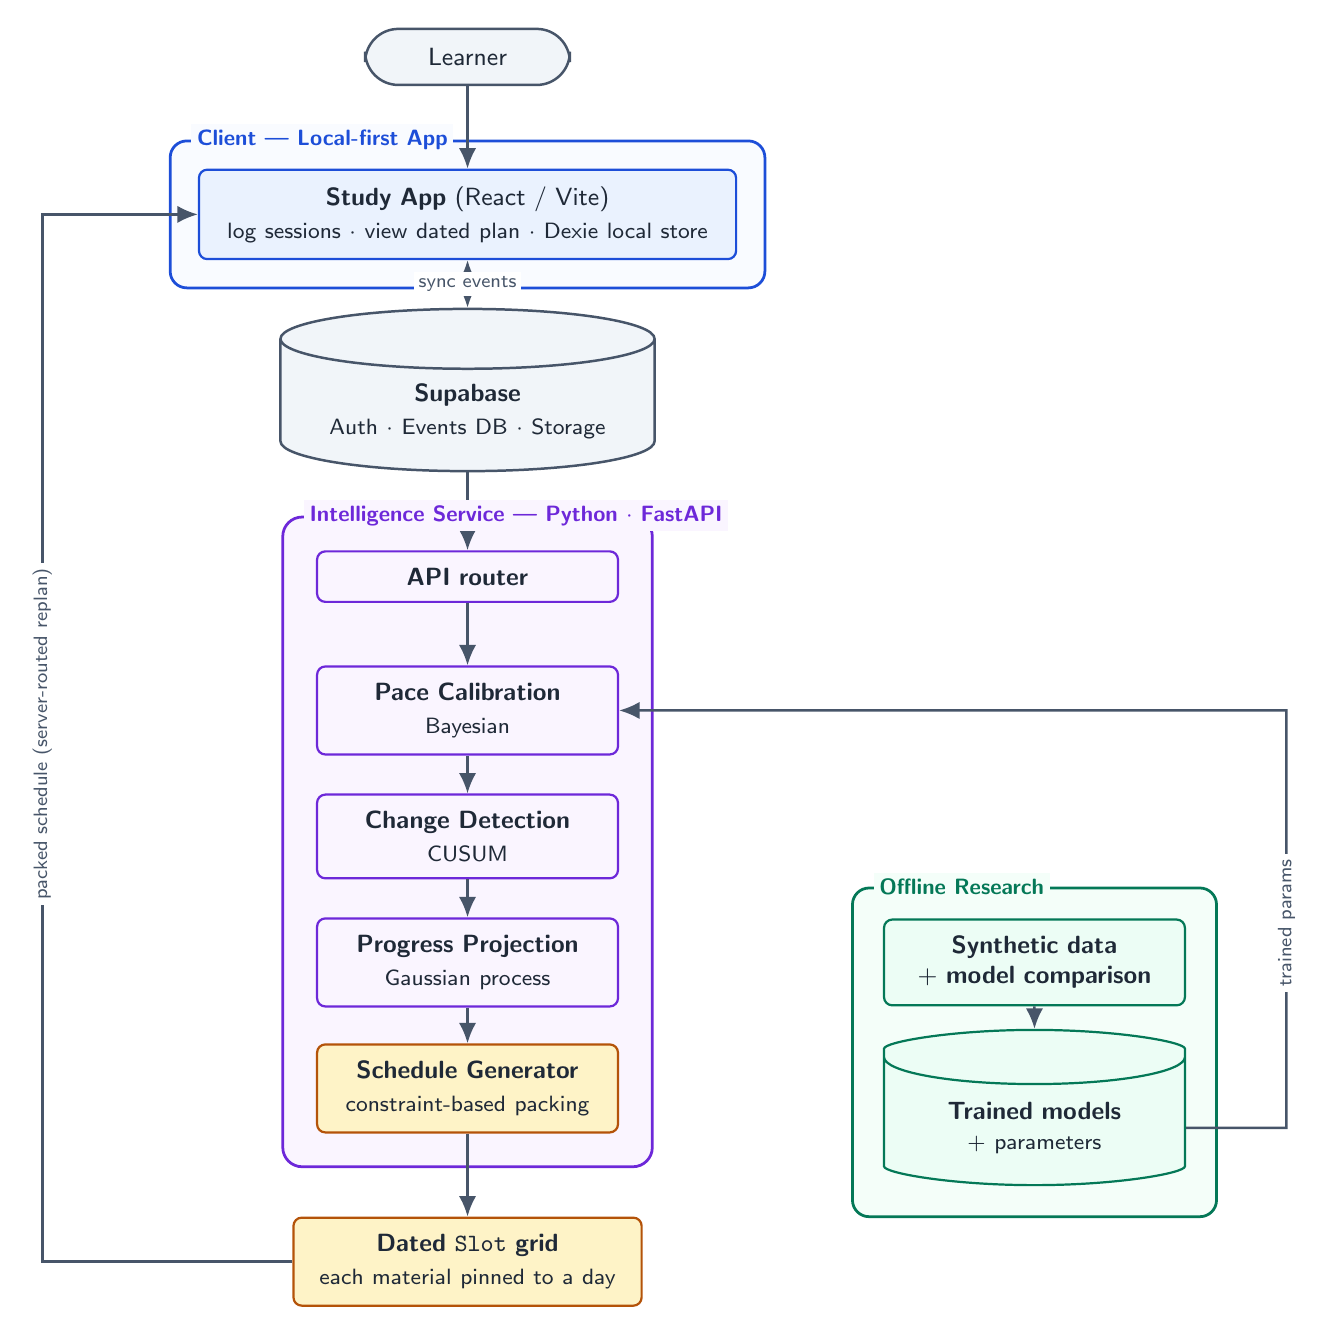
\begin{tikzpicture}[
  font=\small,
  every node/.style={text=inkText},
  box/.style={rounded corners=3pt, draw, line width=0.8pt, align=center,
              inner sep=6pt, text width=3.4cm, fill=white},
  proc/.style={box, draw=blueStroke, fill=paFill},
  svc/.style={box, draw=purpStroke, fill=purpFill},
  outbox/.style={box, draw=amber, fill=amberFill, text width=4.0cm},
  hub/.style={cylinder, shape border rotate=90, aspect=0.16, draw=slate,
              line width=0.9pt, fill=slateFill, align=center, inner sep=5pt,
              text width=4.4cm, minimum height=1.4cm},
  actor/.style={rounded corners=12pt, draw=slate, line width=0.9pt,
                fill=slateFill, align=center, inner sep=7pt, minimum width=2.6cm},
  res/.style={box, draw=greenStroke, fill=greenFill, text width=3.4cm},
  title/.style={font=\footnotesize\bfseries},
  flow/.style={-{Latex[length=2.6mm,width=2.2mm]}, line width=0.9pt, draw=slate},
  flowbi/.style={{Latex[length=2.6mm,width=2.2mm]}-{Latex[length=2.6mm,width=2.2mm]},
                 line width=0.9pt, draw=slate},
  lbl/.style={font=\scriptsize, fill=white, inner sep=1.8pt, text=slate},
]

% ---------------- NODES (absolute grid) ----------------
\node[actor] (LEARNER) at (2,16.2) {Learner};
\node[proc, text width=6.4cm] (APP) at (2,14.2)
  {\textbf{Study App} (React / Vite)\\[1pt]\footnotesize log sessions $\cdot$ view dated plan $\cdot$ Dexie local store};
\node[hub] (SB) at (2,11.7) {\textbf{Supabase}\\[1pt]\footnotesize Auth $\cdot$ Events DB $\cdot$ Storage};
\node[svc] (ROUTER) at (2,9.6) {\textbf{API router}};
\node[svc] (CAL) at (2,7.9) {\textbf{Pace Calibration}\\[1pt]\footnotesize Bayesian};
\node[svc] (DET) at (2,6.3) {\textbf{Change Detection}\\[1pt]\footnotesize CUSUM};
\node[svc] (PROJ) at (2,4.7) {\textbf{Progress Projection}\\[1pt]\footnotesize Gaussian process};
\node[svc, draw=amber, fill=amberFill] (SCH) at (2,3.1)
  {\textbf{Schedule Generator}\\[1pt]\footnotesize constraint-based packing};
\node[outbox] (SLOT) at (2,0.9) {\textbf{Dated \texttt{Slot} grid}\\[1pt]\footnotesize each material pinned to a day};

\node[res] (PIPE) at (9.2,4.7) {\textbf{Synthetic data}\\\textbf{$+$ model comparison}};
\node[res, cylinder, shape border rotate=90, aspect=0.18, minimum height=1.2cm] (MODELS)
  at (9.2,2.6) {\textbf{Trained models}\\\footnotesize $+$ parameters};

% ---------------- CONTAINERS (background) ----------------
\begin{scope}[on background layer]
  \node[draw=blueStroke, line width=1pt, rounded corners=6pt, fill=blueFill!40,
        fit=(APP), inner sep=10pt] (clientBox) {};
  \node[draw=purpStroke, line width=1pt, rounded corners=7pt, fill=purpFill,
        fit=(ROUTER)(CAL)(DET)(PROJ)(SCH), inner sep=12pt] (svcBox) {};
  \node[draw=greenStroke, line width=1pt, rounded corners=6pt, fill=greenFill!60,
        fit=(PIPE)(MODELS), inner sep=11pt] (resBox) {};
\end{scope}

% ---------------- EDGES ----------------
\draw[flow] (LEARNER) -- (APP);
\draw[flowbi] (APP) -- (SB) node[lbl, midway]{sync events};
\draw[flow] (SB) -- (ROUTER) node[lbl, midway]{events};
\draw[flow] (ROUTER) -- (CAL);
\draw[flow] (CAL) -- (DET);
\draw[flow] (DET) -- (PROJ);
\draw[flow] (PROJ) -- (SCH);
\draw[flow] (SCH) -- (SLOT);
% packed schedule returns to the app (far-left lane)
\draw[flow] (SLOT.west) -- (-3.4,0.9) -- (-3.4,14.2) -- (APP.west);
\node[lbl, rotate=90] at (-3.4,7.6) {packed schedule (server-routed replan)};
% research feeds the engines
\draw[flow] (PIPE) -- (MODELS);
\draw[flow] (MODELS.east) -- (12.4,2.6) -- (12.4,7.9) -- (CAL.east);
\node[lbl, rotate=90] at (12.4,5.2) {trained params};

% ---------------- CONTAINER TITLES (on top) ----------------
\node[title, text=blueStroke, fill=blueFill!40, inner sep=2pt, anchor=west]
      at ([xshift=8pt]clientBox.north west) {Client --- Local-first App};
\node[title, text=purpStroke, fill=purpFill, inner sep=2pt, anchor=west]
      at ([xshift=8pt]svcBox.north west) {Intelligence Service --- Python $\cdot$ FastAPI};
\node[title, text=greenStroke, fill=greenFill!60, inner sep=2pt, anchor=west]
      at ([xshift=8pt]resBox.north west) {Offline Research};
\end{tikzpicture}
\end{document}
